\section{Results}\label{Sect_Results}
In this section, we analyze the results of all three model iterations. For the first two versions, we show the prediction error on the ultimate for each \texttt{leaf} and province, while for the third version we only give the average monthly error. It should be noted that we only show the ultimate predictions for claims pending in 2017 and 2018, although we use the incurred as of March 2020. Pending claims in December 2018 had more than 14 months to develop to the ultimate. 
\subsection{First model version: Historical pending claims}
	\paragraph{Quebec:}
		For the first model, the average monthly prediction error is $957,758 \$$, based on a total volume of about 100 million \$. Figure \ref{Fig_QC_current_er_by_month} shows that the error has a light seasonal pattern. In winter, we tend to slightly underestimate, while in most months we overestimate the ultimate loss. The seasonality is difficult to confirm, since we only have 2 years of fully credible data. The error does not seem to be all random and thus should be further investigated. We do notice less cyclic pattern when using a lag and period length which includes the same month of the previous year. However, it does not neutralize it and actually increases the overall error.
		\begin{figure}[H]
			\begin{center}
				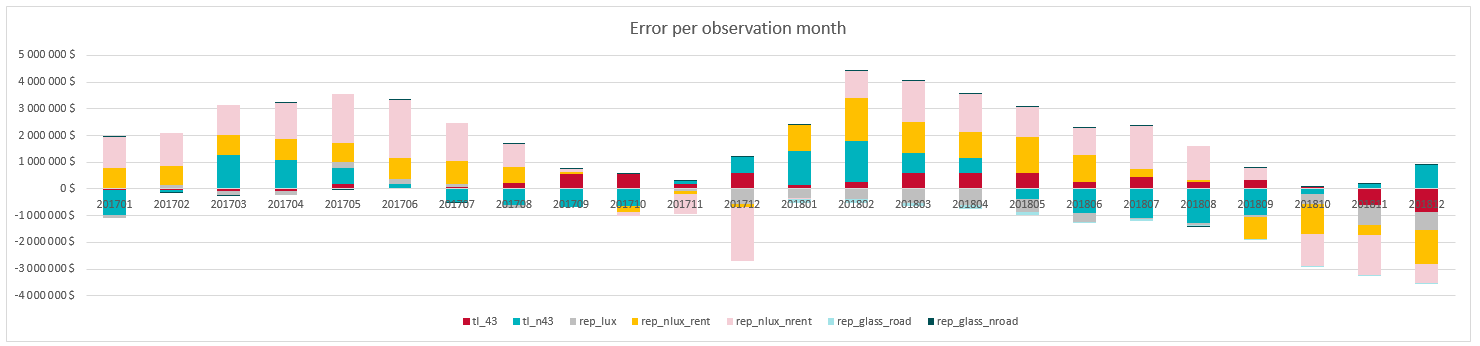
\includegraphics[scale=0.4]{Graphiques/QC_current_model_by_month} 
				\renewcommand{\figurename}{Figure}
				\caption[Quebec version one model error]{Quebec "Historical pending claims" model, prediction error by observation month}\label{Fig_QC_current_er_by_month}
			\end{center}
		\end{figure}
		Figure \ref{Fig_QC_current_er_boxplot} indicates that the largest proportion of error comes from \texttt{tl\_n43} and \texttt{rep\_nlux\_nrent}. These two \texttt{leaf} are also the largest in terms of volume. 
		\begin{figure}[H]
			\begin{center}
				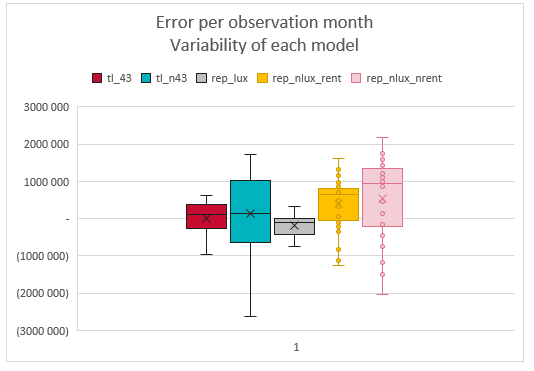
\includegraphics[scale=0.4]{Graphiques/QC_current_model_mustach} 
				\renewcommand{\figurename}{Figure}
				\caption[Quebec version one model error - boxplot]{Quebec "Historical pending claims" model, monthly prediction error boxplot}\label{Fig_QC_current_er_boxplot}
			\end{center}
		\end{figure}
	
	\paragraph{Ontario:}
		In Ontario, the model has the tendency to underestimate the ultimate amount. The average error per observation month shown in figure \ref{Fig_ON_current_er_by_month} is at $-4,632,282\$ $.from the total volume of 100 million \$. Specifically, the winter proves difficult for the model. We are currently investigating this issue, but it might be related to the lag we use and/or the trends observed in the data.
		\begin{figure}[H]
			\begin{center}
				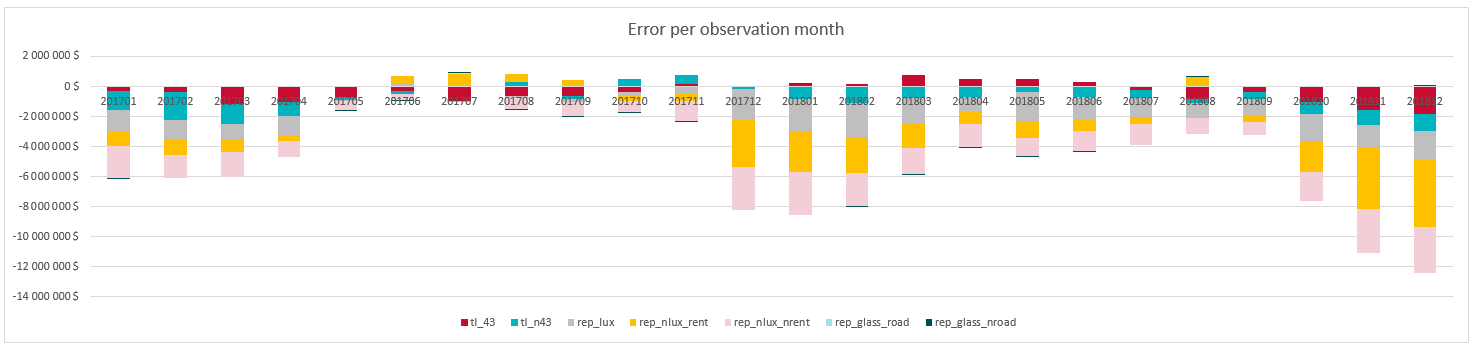
\includegraphics[scale=0.4]{Graphiques/ON_current_model_by_month} 
				\renewcommand{\figurename}{Figure}
				\caption[Ontario version one model error]{Ontario "Historical pending claims" model, prediction error by observation month}\label{Fig_ON_current_er_by_month}
			\end{center}
		\end{figure}
		\begin{figure}[H]
			\begin{center}
				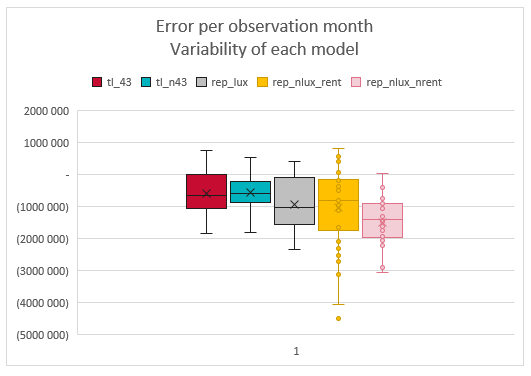
\includegraphics[scale=0.4]{Graphiques/ON_current_model_mustach} 
				\renewcommand{\figurename}{Figure}
				\caption[Ontario version one model error - boxplot]{Ontario "Historical pending claims" model, monthly prediction error boxplot}\label{Fig_ON_current_er_boxplot}
			\end{center}
		\end{figure}
	\paragraph{Alberta:}
		The average monthly prediction error amounts to $3,547,626\$ $ on a total volume of about 80 million \$. There is no clear seasonal pattern. However the model constantly overestimates. The cause of the overestimation is the subrogation, which even after 12 months is not completed. We found about 10\% of the claims in Alberta still receive recovery payments after 12 months. Figure \ref{Fig_AB_current_er_boxplot} shows that \texttt{rep\_nlux\_rent} is the biggest source of error for this model.   
		\begin{figure}[H]
			\begin{center}
				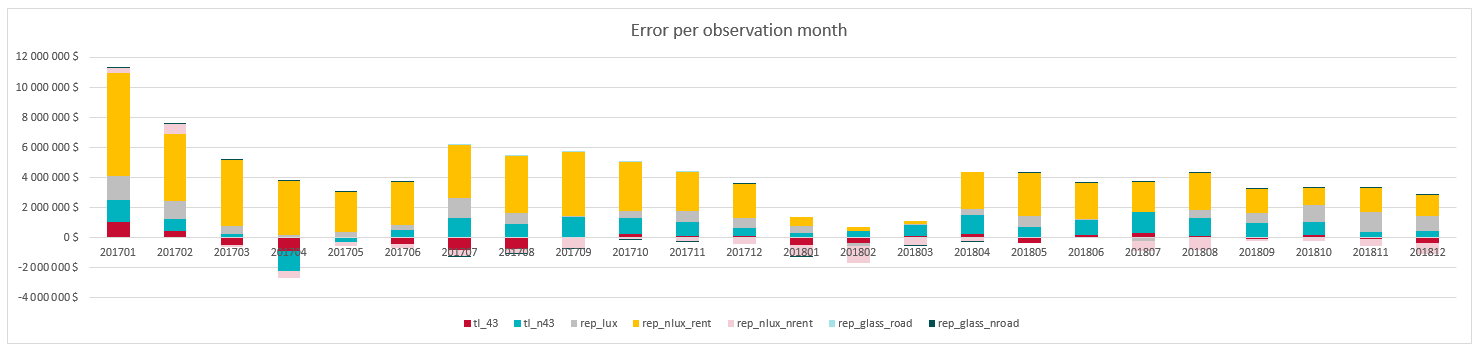
\includegraphics[scale=0.4]{Graphiques/AB_current_model_by_month} 
				\renewcommand{\figurename}{Figure}
				\caption[Alberta version one model error]{Alberta "Historical pending claims" model, prediction error by observation month}\label{Fig_AB_current_er_by_month}
			\end{center}
		\end{figure}
		\begin{figure}[H]
			\begin{center}
				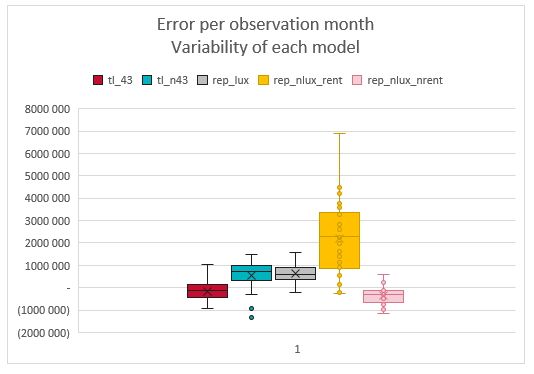
\includegraphics[scale=0.4]{Graphiques/AB_current_model_mustach} 
				\renewcommand{\figurename}{Figure}
				\caption[Alberta version one model error - boxplot]{Alberta "Historical pending claims" model, monthly prediction error boxplot}\label{Fig_AB_current_er_boxplot}
			\end{center}
		\end{figure}
	In section \ref{Section_dataAnalysis}, it was shown that the ALAE might have an impact on the model. However, the model uses a factor proportionnal to the ultimate including ALAE. If the ALAE to loss ratio is stable in time, the factor should account for the ALAE. Thus, the instability of the ALAE to loss ratio observed in the data could cause between 0.2 to 1\% of estimation error.
		
	Overall, when combining all results we can observe that Onatrio and Alberta almost equalize. Figure \ref{Fig_IBNER_preds} shows the results for the December 2019 model (upper graph) and the current model (lower graph). The current model is a significant improvement over the previous model. The December 2019 model uses a different lag than the March 2020 version, as mentioned in section \ref{Sect_dec_march}. The error is rarely greater than 2 million \$. However, the red square indicates a zone of bad predictions amounting to error as high as 18 million \$. One should note that the real IBNER after February 2019 is not reliable, since it is not yet fully developed in some cases.
	
	\begin{figure}[H]
		\begin{center}
			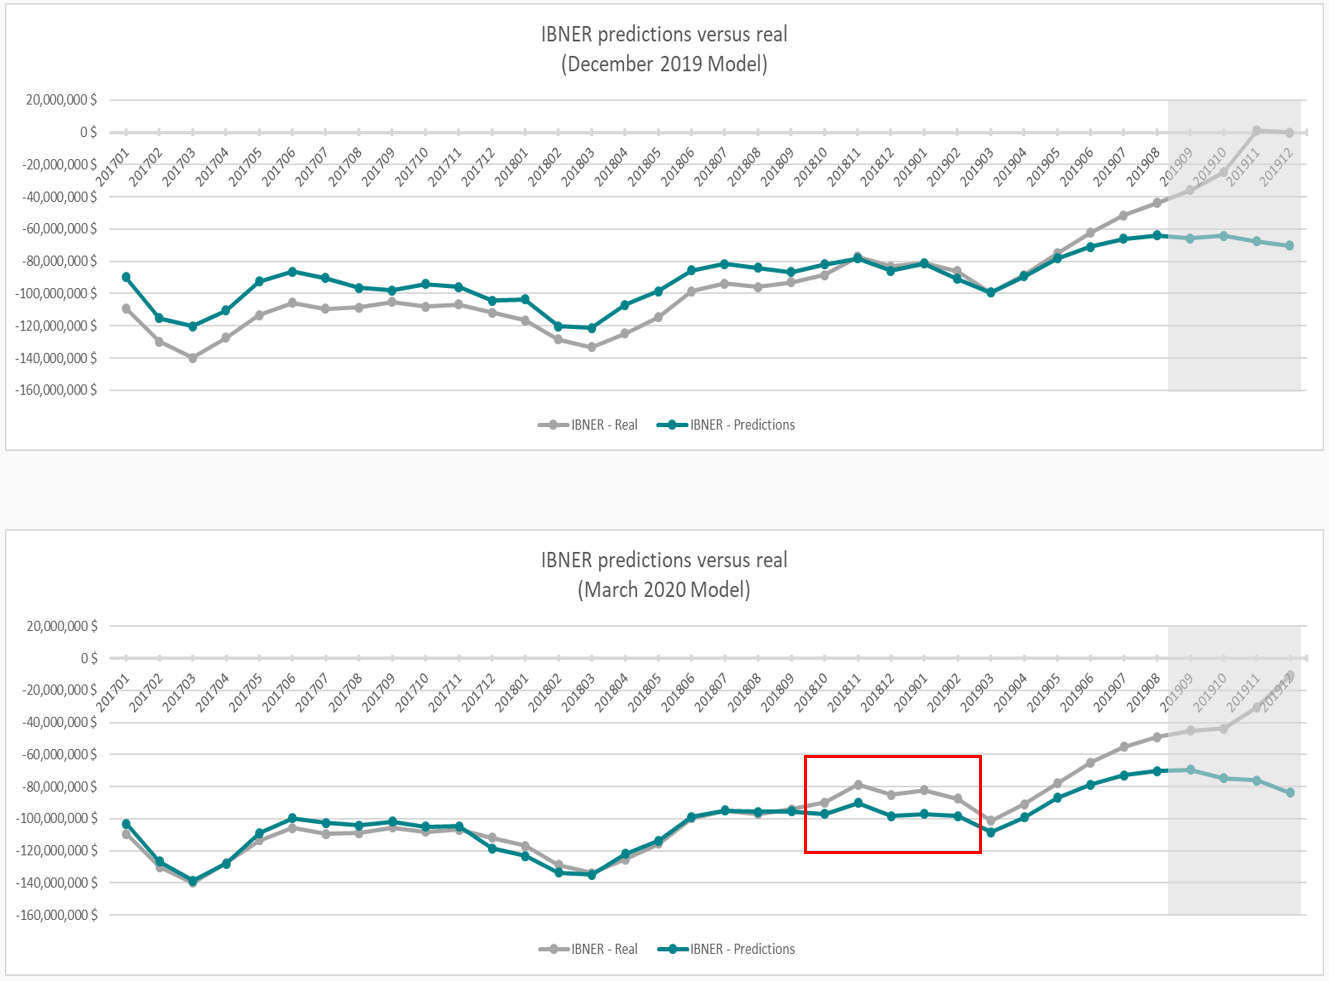
\includegraphics[scale=0.4]{Graphiques/JAN_vs_MARCH} 
			\renewcommand{\figurename}{Figure}
			\caption[IBNER prediction vs real IBNER]{IBNER prediction vs real IBNER ($IBNER_i$ from definition \ref{Def_IBNER}, for $i= 201701,\dots,201812$)}\label{Fig_IBNER_preds}
		\end{center}
	\end{figure}

\subsection{Second model version: Historical pending but now closed claims}
	Excluding open claims in the factor calculations has a strong impact on the model. The average monthly errors are $-1,379,997 \$ $, $-5,134,386 \$ $ and $-431,989\$ $, for Quebec, Ontario and Alberta respectively. This model has a strong tendency to underestimate. Albeit, for Alberta, when looking at the figure \ref{Fig_AB_closedonly_er_by_month}, the results are considerably better than the first model version. Adding open claims seems to multiply the error by a factor of 10. This indicated that once a claim is closed, the subrogation process seems to also be finished or partly finished. For the other two provinces, it shows that adding open claims captures something we are not yet able to fully explain. The issue might be related to the imputation method and observed trends.
		\begin{figure}[H]
			\begin{center}
				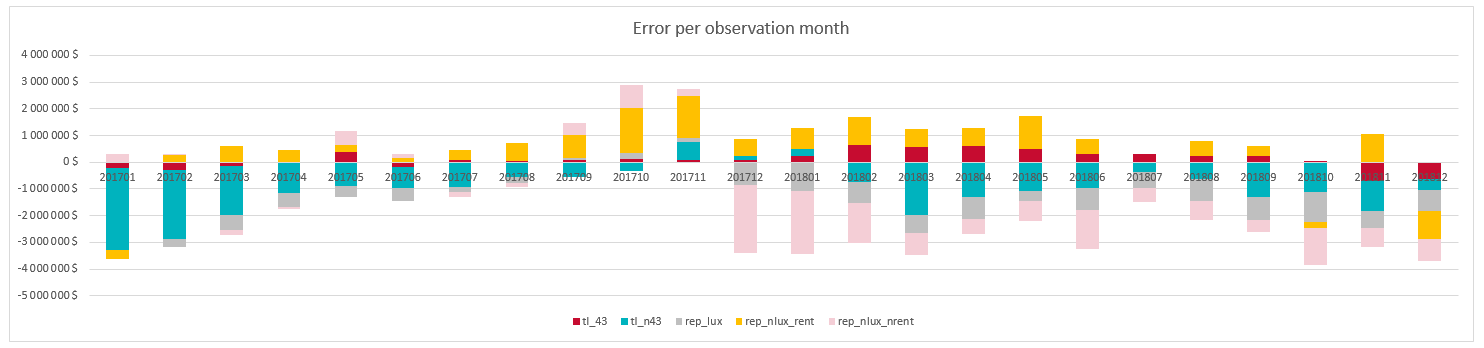
\includegraphics[scale=0.4]{Graphiques/QC_closedonly_model_by_month} 
				\renewcommand{\figurename}{Figure}
				\caption[Quebec version two model error]{Quebec "Historical pending but now closed claims" model, prediction error by observation month}\label{Fig_QC_closedonly_er_by_month}
			\end{center}
		\end{figure}
		\begin{figure}[H]
			\begin{center}
				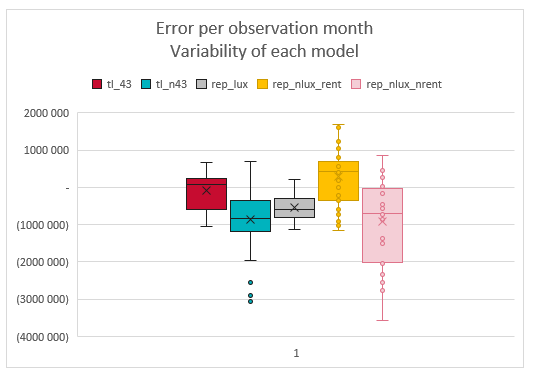
\includegraphics[scale=0.4]{Graphiques/QC_closedonly_model_mustach} 
				\renewcommand{\figurename}{Figure}
				\caption[Quebec version two model error - boxplot]{Quebec "Historical pending but now closed claims" model, monthly prediction error boxplot}\label{Fig_QC_closedonly_er_boxplot}
			\end{center}
		\end{figure}

		\begin{figure}[H]
			\begin{center}
				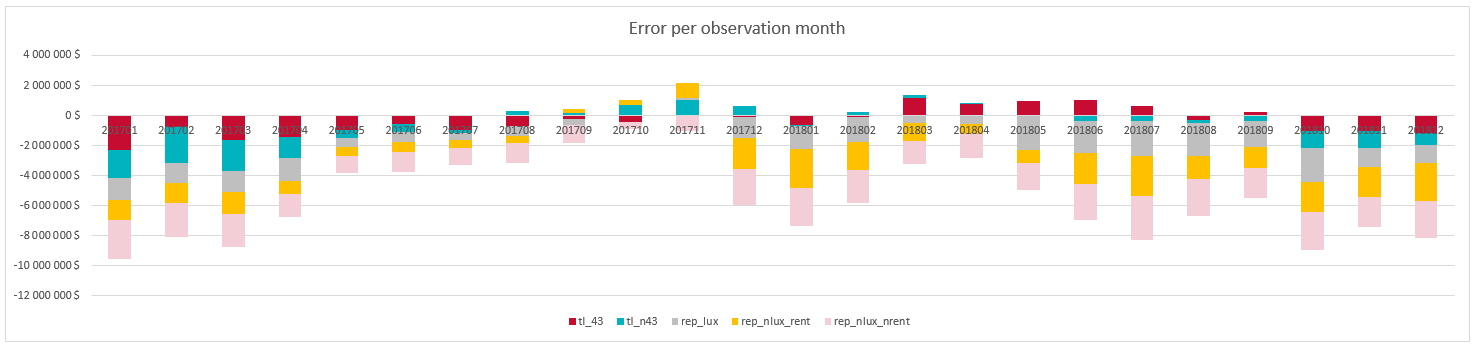
\includegraphics[scale=0.4]{Graphiques/ON_closedonly_model_by_month} 
				\renewcommand{\figurename}{Figure}
				\caption[Ontario version two model error]{Ontario "Historical pending but now closed claims" model, prediction error by observation month}\label{Fig_ON_closedonly_er_by_month}
			\end{center}
		\end{figure}
		\begin{figure}[H]
			\begin{center}
				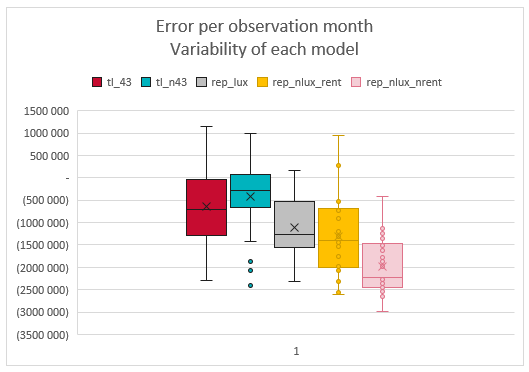
\includegraphics[scale=0.4]{Graphiques/ON_closedonly_model_mustach} 
				\renewcommand{\figurename}{Figure}
				\caption[Ontario version two model error - boxplot]{Ontario "Historical pending but now closed claims" model, monthly prediction error boxplot}\label{Fig_ON_closedonly_er_boxplot}
			\end{center}
		\end{figure}


		\begin{figure}[H]
			\begin{center}
				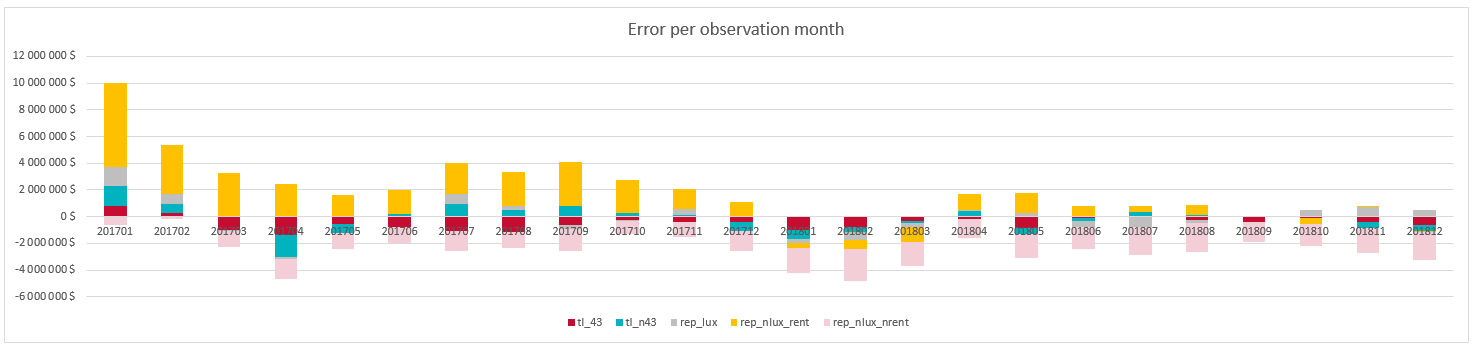
\includegraphics[scale=0.4]{Graphiques/AB_closedonly_model_by_month} 
				\renewcommand{\figurename}{Figure}
				\caption[Alberta version two model error]{Alberta "Historical pending but now closed claims" model, prediction error by observation month}\label{Fig_AB_closedonly_er_by_month}
			\end{center}
		\end{figure}
		\begin{figure}[H]
			\begin{center}
				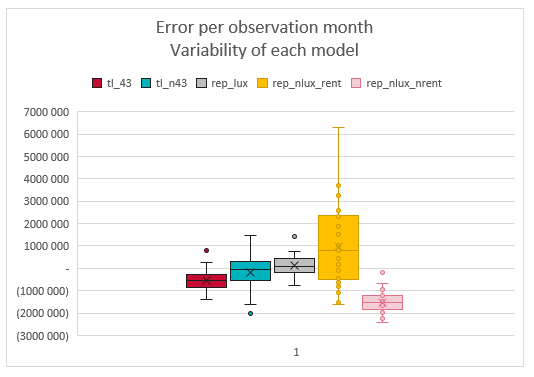
\includegraphics[scale=0.4]{Graphiques/AB_closedonly_model_mustach} 
				\renewcommand{\figurename}{Figure}
				\caption[Alberta version two model error - boxplot]{Alberta "Historical pending but now closed claims" model, monthly prediction error boxplot}\label{Fig_AB_closedonly_er_boxplot}
			\end{center}
		\end{figure}
	
\subsection{Third model version: Historical closed claims }
	Lastly, the third model version seems not to function as well as expected. Quebec has an average monthly error of $-7,196,717 \$ $, Ontario of $-13,153,106 \$ $ and Alberta of $4,148,104 \$ $. One issue with this model is related to the claims in the window. While the two previous model uses a small window of pending claims, this model uses all claims that closed in the time window. Thus, we are using claims that can be very old relative to the observation month or claims that are not representative of current pending claims. 
	
	
		 